\documentclass[twocolumn,10pt,a4j]{ltjsarticle}
\usepackage{kougai}

\title{研究報告}
\author{2132100 中野 星花  指導教員 須田 宇宙 准教授}
\date{}

\begin{document}

\maketitle

\section{はじめに}
一般的な教育は,教師中心の講義形式であるため受動的な学習になりがちである.しかし、社会全体で自ら学習し,課題を見つけ解決する能力が求められている.そのため,文部科学省は2020年度に改定された学習指導要領で主体的・対話的な学びとしてアクティブラーニングを推奨した.その一つに他者説明という学習方法がある.学習内容を他者に説明することで,知識を整理し,質問に答えることで新たな視点を得ることができるため自身の理解度や説明方法の改善に効果が期待できる.
しかしこの学習方法には,説明を聞く人の理解状態を推論し,教えたことのフィードバックが必要になる点が課題である.これまでにこれらの課題に着目したアクティブラーニングの分野の研究のほとんどが,説明内容を吟味するために教師の介入が必要であった点に効率性に課題が残ると考える.
また,フィードバックを求める場としてAIを活用した研究では,記録した会話の文章を分析するために活用されているため,AIと対話している訳ではない.そこで,本研究では,AIに対して学習内容を説明させることで学習者自身の理解度を認識させる学習方法を提案する.

\section{他者説明とは}
学習内容は他の人に教えたときにより定着率が高くなると言われている.
教えるという技術は,正解を答えるだけではなく,ものごとの仕組みや原理を伝え,その知識や技能が教える対象者にも利用できるようにすることである.
たとえばものごとの仕組みや原理を伝えるためには,どのような知識が必要になるのかを考え,情報の整理・構造化をし,相手が理解出来るまでの試行錯誤が求められる.
従って,このプロセスを用いた学習方法 は,学習者自身があいまいにしている部分を再確認・再学習 する機会を提供することができる点で,学習方略として有効な手段と言える.


\section{研究の構想}
本研究では,対話形式の他者説明において,学習者が知識を整理し,より理解が深まるような質問内容やシナリオの考案を目的とする.会話形式の他者説明の手法を図1に示す.また,学習者の回答に対する質問内容を簡潔に表1に示す.学習者の回答にもとづく質問内容を分類することで,目標とする理解を促進させるようなシナリオになると考えた.
また,このシステムの対象者によって質問内容の難度が変わる点も考慮する必要があると考えた.

\begin{figure}[h]
\begin{center}
 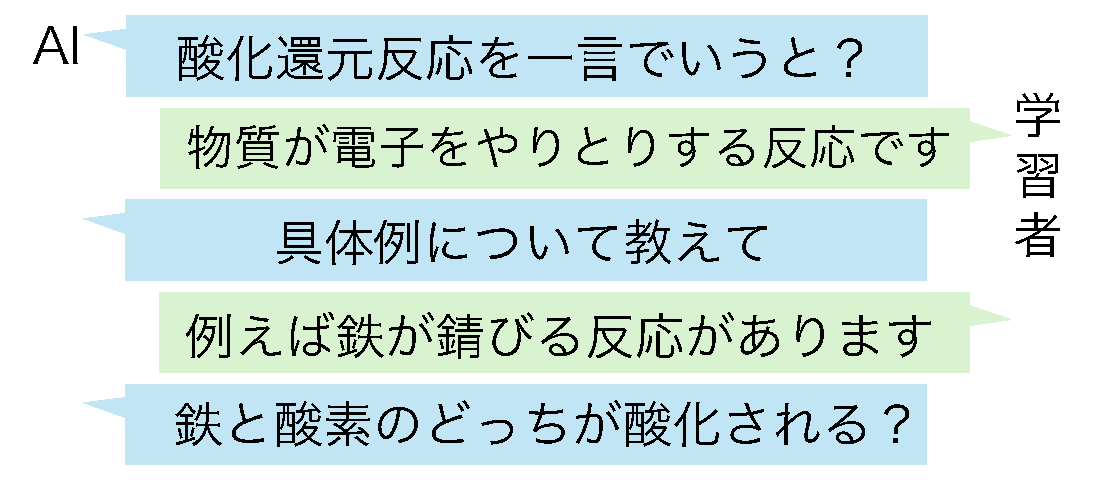
\includegraphics[clip,width=55mm,height=40mm]{talk_log.pdf}
\end{center}
 \caption{対話形式の他者説明}
 \label{fig:図形}
\end{figure}

\begin{table}[h]
\begin{center}
\label{tab:hogehoge}
\begin{tabular}{ll}

\hline

        \multicolumn{1}{l}{学習者の回答} & \multicolumn{1}{l}{質問内容}  \\  \hline \hline 
        \multicolumn{1}{l}{間違いは言っていない} & \multicolumn{1}{l}{具体例を質問} \\ 
         \multicolumn{1}{l}{} & \multicolumn{1}{l}{回答から質問} \\ 
          \multicolumn{1}{l}{} & \multicolumn{1}{l}{まだ聴いてないことを質問} \\ 
          \multicolumn{1}{l}{} & \multicolumn{1}{l}{間違いを再確認} \\ \hline
          \multicolumn{1}{l}{間違いを含む} & \multicolumn{1}{l}{間違った単語を質問} \\
          \multicolumn{1}{l}{} & \multicolumn{1}{l}{聞き返す} \\ \hline
           \multicolumn{1}{l}{間違っている,答えられない} & \multicolumn{1}{l}{回答から質問} \\
          \multicolumn{1}{l}{} & \multicolumn{1}{l}{関連ワードを質問} \\ 
          \multicolumn{1}{l}{} & \multicolumn{1}{l}{説明} \\ \hline
                 
\end{tabular}
\end{center}
\caption{表のタイトル}
\end{table}

\section{今後の予定}
表1をもとに被験者に他者説明をさせ、このシナリオが有効かどうか検証する.





\begin{thebibliography}{99}
\bibitem{suda2018} 須田宇宙: ``音響科学e-Learning教材'', \url{https://www.sudalab.net/}, 2018/7/19参照
\end{thebibliography}

\end{document}
